\documentclass[12pt]{article}
\usepackage{graphicx}
\usepackage {color}
\usepackage{pdfpages}
\usepackage{float}
\usepackage{changebar}
\usepackage{enumitem,amssymb}
\renewcommand{\familydefault}{\sfdefault}
\usepackage[margin=1.2in]{geometry}
\usepackage{graphicx}
\usepackage{wrapfig}
\usepackage[super]{cite}
\usepackage{subcaption}
\usepackage[table]{xcolor}
\usepackage{amsmath}
\usepackage[sort, numbers]{natbib}
\usepackage{multirow}
\usepackage{tabularx}
\usepackage{siunitx}
\usepackage{matlab-prettifier}
%%%%%%%%%%%%Defining the margins %%%%%%%%%%%%%%%%%%%%%
\textheight 9.in
\textwidth 6.5in
\topmargin -.5in
\oddsidemargin 0in
\setlength{\parskip}{\smallskipamount}

%%%%%%%%%%%%%%Specific Commands %%%%%%%%%%%%%%%%%%
\newcommand{\eg}{{\em e.g.,}}
\newcommand{\ie}{{\em i.e.,}}
\newcommand{\etc}{{\em etc.,}}
\newcommand{\etal}{{\em et al.}}
\newcommand{\degrees}{{$^{\circ}$}}
\newcommand{\fig}[1]{\textbf{Figure #1}}

%%%%%%%%%%%%%%%%%%%%%%%%%%%% Setting to control figure placement
% These determine the rules used to place floating objects like figures 
% They are only guides, but read the manual to see the effect of each.
\renewcommand{\topfraction}{.9}
\renewcommand{\bottomfraction}{.9}
\renewcommand{\textfraction}{.1}
\renewcommand{\familydefault}{\sfdefault} %setting the san serif font

%%%%%%%%%%%%%%%%%%%%%%%% Line spacing
% Use the following command for ``double'' spacing
%\setlength{\baselineskip}{1.2\baselineskip}
% and this one for an acceptable NIH spacing of 6lpi based on 11pt
%\setlength{\baselineskip}{.9\baselineskip}
% The baselineskip does not appear to work when we include a maketitle
% command in the main file.  Something there must set the line spacing
% If we use this next command, then things seem to work.
\renewcommand{\baselinestretch}{.9}

\setcounter{secnumdepth}{0} %make no numbers but have a table of contents


\begin{document}

\title{HW 3: Medical Imaging Systems}
\author{Jake Bergquist, u6010393 }
\maketitle

\section{Q1}
\noindent\textbf{a: }
For question 1 I have re-drawn the sequence on the attached pages as can be seen in Drawing 1.  The colors used correspond to the traversal of the K space in Drawing 2. On Drawing 2 a solid line designates a sampling and a dotted line signifies a traversal of the K space without sampling. The $G_X$ axis is shown in red and the $G_Y$ axis is shown in blue. The numbers labeling the traversals of the K space on Drawing 2 correspond to the different pulses in the sequence depicted in Drawing 1. In each case all of the $G_X$ pulses are assumed to be equal (having equal area under the curve) except for the first $G_X$ pulse which is assumed to have a an area under the curve that is half that of the subsequent ones. All of the $G_Y$ pulses are assumed to have equal magnitude of area under the curve (some being negative). All traversals of the K space are thus given in a unit length. Following the trajectory from the origin first there is a dephasing pulse on $G_X$ (1) that moves us to a position in the positive direction on the $G_X$ axis of the K space to (1,0). Then there is a 180 pulse (2) that causes a traversal to a place on the negative $G_X$ axis to (-1,0). Next there is a $G_y$ pulse (3) that moves us to (-1.1) in the K space, followed by the first acquisition pulse (4) which acquires samples as we move from (-1,1) to (1,1). Next there is an inversion (5) that moves us to (-1,-1) followed by a negative $G_Y$ pulse (6) that moves us to (-1,-2). Then another acquisition(7) as we move to (-1,-2) to (1,-2). Then an inversion (8) to (-1,2). Then a positive $G_Y$ (9) to move to (-1,3). Then an acquisition (10) as we move to (1,3). Then an inversion (11) to (-1,-3). Then a negative $G_Y$ (12) to move to (-1,-4). Then the final acquisition as we move to (1,-4).

\noindent\textbf{b: }


\begin{lstlisting}[style=Matlab-editor]
%Q5
TI = [50 100 200 400 800 1600];
tissue1 = [-889 -684 -461 99.4 385 780];
tissue2 = [-261 -217 -108 118 254 339];

objFunc_tiss1 = @(param) LongMagIntensity(TI,tissue1,param);
optParams_tiss1 = fminsearch(objFunc_tiss1,[500,500]);
figure(1);clf();hold on;
plot(TI,tissue1,'r','linewidth',2);
plot([50:1600],optParams_tiss1(1).*(1-2*exp(-[50:1600]/optParams_tiss1(2))),'b','linewidth',2);
xlabel('TI (msec)');ylabel('intensity');set(gca,'fontsize',18);

objFunc_tiss2 = @(param) LongMagIntensity(TI,tissue2,param);
optParams_tiss2 = fminsearch(objFunc_tiss2,[500,500]);
figure(2);clf();hold on;
plot(TI,tissue2,'r','linewidth',2);
plot([50:1600],optParams_tiss2(1).*(1-2*exp(-[50:1600]/optParams_tiss2(2))),'b','linewidth',2);
xlabel('TI (msec)');ylabel('intensity');set(gca,'fontsize',18);

function cost = LongMagIntensity(TI,m,param)
M0 = param(1);
T1 = param(2);
cost = sum((m - M0 * (1 - 2*exp(-TI/T1))).^2);

end
\end{lstlisting}





\end{document}



\begin{figure}[H]
	\centering
	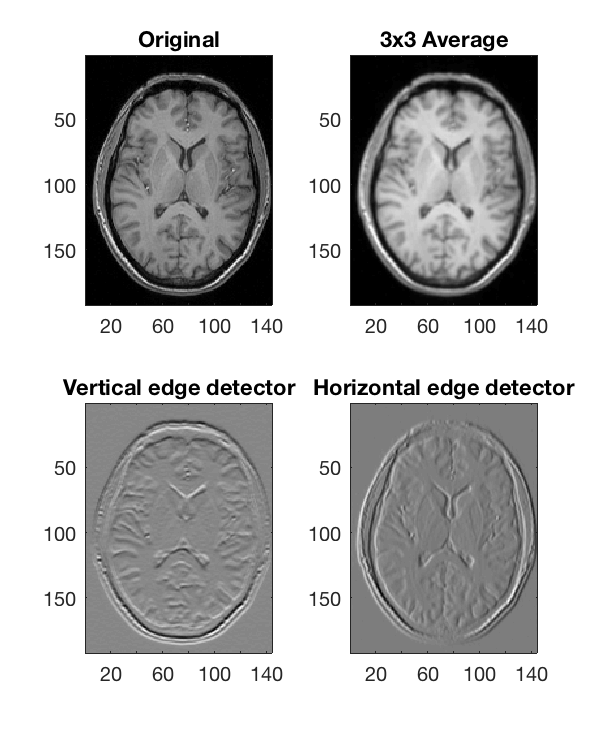
\includegraphics[width=\textwidth]{Figures/convs.png}
	\caption{}
	\label{Fig:conv}
\end{figure}






